% !TEX root = ../main.tex
\paragraph{CS-Studio}
\label{par::cs_studio}
    The Graphical User Interface (GUI) of CLAS12 EPICS is built on the Control System Studio (CS-Studio) toolkit.
    CS-Studio is specifically designed for monitoring and operating large-scale control systems and is based on the eclipse Rich Client Platform (RCP) framework \cite{kasemir2007}.
    To integrate the RG-E target system into CLAS12 EPICS, a CS-Studio screen was developed.

    Below is a list of the requirements that the screen needed to fulfil.
    These requirements were derived from the specifications of the physics experiments as well as the needs of the electronics team responsible for the target system.

    \begin{itemize}
        \item
            Buttons to move the target band to the targets and a home location.
        \item
            A Button to stop the target band in case of emergency.
        \item
            A status check on the position of the target band.
        \item
            Alarm handling for the case when the band moves beyond low and high limits.
        \item
            Alarm handling for the IOC and communication problems.
    \end{itemize}

    \begin{figure}[b!]
        \centering\frame{
        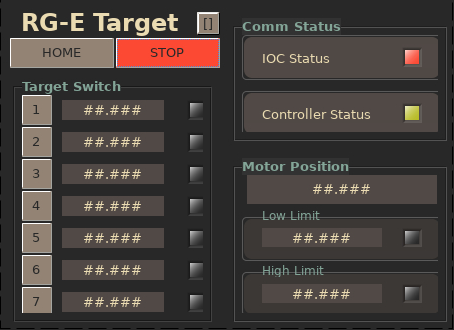
\includegraphics[]{312motorx_rge.png}}
        \caption[RG-E CS-Studio main screen]{RG-E CS-Studio main screen. The HOME and A, B, C, etc buttons move the target strip to the corresponding location, the STOP button is an emergency, instant stop of the target system, and the Motor Screens button allows the user to open additional motor screens.
        Source: Own Elaboration using \hyperlink{controlsystemstudio.org/}{CS-Studio}.}
        \label{fig::rge_motorx}
    \end{figure}

The implemented screen, shown in Figure \ref{fig::rge_motorx}, incorporates these requirements.
    Along with the buttons, text displays indicate the position of each target within the band.
    Adjacent LED displays illuminate green when the band position aligns with the target position, within the tolerance specified in the database.
    Additionally, four LED displays are positioned to the right of the two IOC statuses, as well as the low and high limits.
    These LEDs indicate alarm conditions and work in conjunction with the CLAS12 Slow Control alarm system to alert the user of any issues.

    Furthermore, in addition to the aforementioned screen, users can access other screens through the Motor Screens menu button.
    These screens are part of the motor EPICS support module and are retained for debugging purposes.
    They include a manual motor movement screen, a motor setup screen, a direct Command Line Interface (CLI) with the motor, and an amplifier configuration screen.
    All of these screens were developed by the Galil EPICS team \cite{farnswort2009}.

    To enhance user experience, the GUI was designed using the Gruvbox colour palette.
    This palette is specifically chosen to ensure that colours are easily distinguishable, with sufficient contrast, while also being visually appealing and comfortable for the eyes.
    The Gruvbox colour palette can be found on GitHub at

    \begin{center}
        \hyperlink{github.com/morhetz/gruvbox}{\texttt{github.com/morhetz/gruvbox}}.
    \end{center}
